\tolerance 500   % Verhindet pingelige "`overfull \hbox"'-Meldungen.

\documentclass[12pt,a4paper,normalheadings,oneside,DIV9,BCOR10mm,listsleft,fleqn,leqno,tablecaptionbelow,abstracton,pointlessnumbers]{scrbook}

\usepackage[T1]{fontenc}
\usepackage[utf8]{inputenc}

%% Einfache Definitionen von Konstanten fuer das gesamte Dokument.
%  Sie werden bspw. beim Aufbau der Titelseite ausgewertet.
\def\titelname    {Detecting Vague Requirements with Machine Learning}
\def\autorforinfo {Leo Hanisch}
\def\email        {leo.hanisch@tum.de}
\def\subjectname  {Prozessmodellierung}	%Beispiel
\def\location     {M\"unchen}
\def\keywordsname {Vague Requirements}			%Beispiel

%% spezifisch fuer eine MA, fuer BA etc. muss das angepasst werden
\def\doctype{Masterarbeit in Informatik}
\def\title{Detecting Vague Requirements with Machine Learning}
\def\titleGer{Detektion von vagen Anforderungen mit maschinellem Lernen}
\def\author{Leo Hanisch}
\def\date{November 15, 2020}

%% Festlegen der Dokumentmetrik
\usepackage[inner=2.5cm,outer=3.5cm,top=1cm,bottom=1cm,includeheadfoot]{geometry}
\usepackage{palatino}
\usepackage{amsmath}
\usepackage{amssymb}
\usepackage{amsthm}
\usepackage{amsbsy}
\usepackage{babel}
\usepackage{paralist}

\usepackage{xspace}

%% Bereich Tabellen
\usepackage{array}
\usepackage{tabularx}
\usepackage{booktabs}
\usepackage{colortbl}
\usepackage{everysel}
\usepackage{framed}
\usepackage{ragged2e}

%% Einbindung von Minitocs
\usepackage{shorttoc}
\usepackage{minitoc}

%% Flexible Tabellenspalten und Kommandos
\newcolumntype{L}{>{\RaggedRight\arraybackslash}X}%
\newcolumntype{C}{>{\Centering\arraybackslash}X}%
\newcolumntype{R}{>{\RaggedLeft\arraybackslash}X}%

\newcommand{\opentableheader}{\toprule}
\newcommand{\closetableheader}{\toprule}

%% actual versions of the listings package:
%% ftp://ftp.dante.de/tex-archive/help/Catalogue/entries/listings.html
\usepackage{listings}
\usepackage{dotnet_new}
\usepackage[pdftex, colorlinks,
            linkcolor=black,
            citecolor=black,
            pagecolor=black,
            filecolor=black,
            urlcolor=black]{hyperref}
\usepackage{graphicx}

\usepackage{bibgerm}
\usepackage{array}
\usepackage{colortbl}
\usepackage{longtable}
\usepackage[final]{pdfpages}

%% Benutzen der Koma-Headings
\usepackage[komastyle]{scrpage2}

%% kompakte Items
\usepackage{paralist}

%% verbatin in footnode
\usepackage{fancyvrb}

\usepackage{natbib}

%% Eigene Packages
%%%
%%% Abk�rzungen
%%%

%%% Referenzierungshilfen


%%% Fachbegriffe
\newcommand{\vmxt}{V-Modell~XT}
\newcommand{\vmx}{V-Modell}




\newcommand{\JEE}{Java~2 Plattform Enterprise Edition}
\newcommand{\JSE}{Java~2 Plattform Standard Edition}
\newcommand{\DOTNET}{.{\@}NET}
\newcommand{\COMPLUS}{COM+}
\newcommand{\Cpp}{C++}
\newcommand{\CSHARP}{C\#}
\newcommand{\ES}{\emph{Enterprise Services}}
\newcommand{\Rem}{\emph{.NET Remoting}}

%%% (kommerzielle) Produkte
\newcommand{\productname}[1]{#1}
\newcommand{\iis}{\productname{IIS}}
\newcommand{\IIS}{\productname{Internet Information Services}}
\newcommand{\VSN}{\productname{Visual Studio.NET}}
\newcommand{\BCB}{\productname{Borland C\#~Builder}}
\newcommand{\BJB}{\productname{Borland JBuilder}}

%%% Makros
\newcommand{\kw}[1]{\texttt{#1}}  % weil ich faul bin...
\newcommand{\method}[1]{Methode \texttt{#1()}}
% etwa: "\method{create}\ zeigt...", nicht: "Die \method{create}"=Methode..."

%%% f�r Bewertungen und Checklisten (zB in Tabellen)

\newcommand{\EVp}{+\xspace}   % +
\newcommand{\EVpp}{++\xspace}   % ++
\newcommand{\EVppp}{+++\xspace}   % +++
\newcommand{\EVm}{--\xspace}   % -
\newcommand{\EVmm}{{--}{--}\xspace}   % --
\newcommand{\EVmmm}{{--}{--}{--}\xspace}   % ---
\newcommand{\EVneutral}{--{\slash}+\xspace}   % -
\newcommand{\CHyes}{\ding{51}}  % yes, Haken
\newcommand{\CHno}{--}  % no


%%% Abk�rzungen - Floskeln
% Die Makros sollten eingesetzt werden, um die W�rter als Abk�rzungen zu nutzen.
% Wenn man also "`vergleiche"' ausgeschrieben haben will, dann muss
% man dieses Wort voll ausgeschreiben.
%
% Der Einsatz ist Geschmacksache, bei einigen Sachen aber sinnvoll.

\newcommand{\vgl}{vgl.\@}               % vergleiche
\newcommand{\etc}{etc.\@}               % Achtung: am Satzende nicht verwenden!
\newcommand{\evtl}{evtl.\@}             % eventuell
\newcommand{\bspw}{bspw.\@}             % beispielsweise
\newcommand{\oa}{o.\,a.\@}              % ...
\newcommand{\zB}{z.\,B.\@}
\newcommand{\zT}{z.\,T.\@}
\newcommand{\zZt}{z.\,Zt.\@}
\newcommand{\ua}{u.\,a.\@}
\newcommand{\ca}{ca.\@}
\newcommand{\dhx}{d.\,h.\@}
\newcommand{\usw}{usw.\@}
\newcommand{\bzw}{bzw.\@}
\newcommand{\bzgl}{bzgl.\@}
\newcommand{\Bzgl}{Bez�glich\@}
\newcommand{\sog}{sog.\@}
\newcommand{\ggf}{ggf.\@}
\newcommand{\Ggf}{Gegebenenfalls}
\newcommand{\vs}{vs.\@}
\newcommand{\engl}{engl.\@}             % englisch (z.B. f�r Wortbedeutungen...)
\newcommand{\inkl}{inkl.\@}
\newcommand{\teilw}{teilw.\@}
\newcommand{\idR}{i.\,d.\,R.\@}
\newcommand{\iS}{i.\,S.\@}
\newcommand{\uU}{u.\,U.\@}
\newcommand{\dW}{des Weiteren}
\newcommand{\DW}{Des Weiteren}
\newcommand{\iFx}{im Folgenden}
\newcommand{\IFx}{Im Folgenden}

%% GKa 2009-06-10: paar weitere commands speziell fuer diesen TR
\newcommand{\PET}{Process Enactment Tool Framework}
\newcommand{\WP}{Werkzeug Provider}
\newcommand{\TP}{Tool Provider}


%%%
%%% Eigene Kommandos und Umgebungen
%%%

% page clearing
\newcommand{\clearemptydoublepage}{%
  \ifthenelse{\boolean{@twoside}}{\newpage{\pagestyle{empty}\cleardoublepage}}%
  {\clearpage}}

%% Farbdefinitionen
%  red, green, blue, white und black stammen aus color.sty
\definecolor{brightgray}{gray}{0.9}
\definecolor{darkgray}{gray}{0.5}
\definecolor{darkgreen}{rgb}{0.0,0.5,0.0}
\definecolor{dg}{rgb}{0.0,0.5,0.0}  %% dark green (Kommentare in listings)
\definecolor{dr}{rgb}{0.5,0.0,0.0}  %% dark red

%% Neuformatierung der Absatztrennung
%  Abs�tze haben 0pt Einzug und sind mit vert. Abstand
%  voneinander separiert
\setlength\parskip{\smallskipamount}
\setlength\parindent{0pt}

%% Redefinition Typewriter Font = kleinere Schrift und Silbentrennung
\renewcommand\texttt[1]{\small\ttfamily\hyphenchar\font=\defaulthyphenchar #1{}\normalsize\rmfamily\hyphenchar\font=\defaulthyphenchar}

%% Festlegen Standard-Listing Schrift
\lstset{language=csharp,extendedchars=true,basicstyle=\footnotesize\ttfamily,commentstyle=\itshape,breaklines=true}

%% Einfaches Umschalten zwischen verschiedenen Programmiersprachen
%  und dem Font, der zur Daterstellung verwendet wird.
%  Parameter:
%  1: Name der Sprache, z.B. csharp
%  2: Name der Fontfamilie, z.B. \ttfamity
%  3: Name der Fontfamilie f�r Kommentare, z.B. \itshape
%
%  Beispiel: \setlistingstyle{csharp}{\ttfamily}{\itshape}
\newcommand{\setlistingstyle}[3]{%
\lstset{language=#1,extendedchars=true,basicstyle=\footnotesize#2,commentstyle=#3,breaklines=true}
}

%% Der Darstellungsstil des Listings wird auf den Standard
%  zur�ckgesetzt
\newcommand{\resetlistingstyle}{%
\lstset{language=csharp,extendedchars=true,basicstyle=\footnotesize\ttfamily,commentstyle=\itshape,breaklines=true}
}

%% Redifinition: Formate und Fonts f�r Unter/�berschriften:
\addtokomafont{caption}{\sffamily\small}
\setkomafont{captionlabel}{\sffamily\bfseries}
\setkomafont{descriptionlabel}{\sffamily\bfseries\small}

%% Gliederung \part wird ohne Pr�fix z.B. "Teil" angezeigt.
\renewcommand*{\partformat}{\thepart\autodot}
\deffootnote{1em}{1em}{\thefootnotemark\ }

%% Neue Theoreme
\newtheoremstyle{style}
   {}                   %Space above
   {}                   %Space below
   {}                   %Body font: original {\normalfont}
   {}                   %Indent amount (empty = no indent,
                           %\parindent = para indent)
   {\normalfont\sffamily}  %Thm head font original {\normalfont\bfseries}
   {:}                     %Punctuation after thm head original :
   {\newline}              %Space after thm head: " " = normal interword
                           %space; \newline = linebreak
   {\textbf{\thmname{#1}\thmnumber{ #2}\thmnote{ (#3)}}}                    
                                        %Thm head spec (can be left empty, meaning
                           %`normal') original {\underline{\thmname{#1}\thmnumber{ #2}\thmnote{ (#3)}}}
 
\theoremstyle{style} 
\newtheorem{defi}{Definition}[chapter]
\newtheorem{bsp}{Example}[chapter]
\newtheorem{softconstraint}{Soft Constraint}[chapter]
\newtheorem{hardconstraint}{Hard Constraint}[chapter]
\newtheorem{anforderung}{Requirement} [chapter]

\newcommand{\betrachtungergebnis}[2]{
	\begin{table}[h!]
	\begin{tabularx}
	{\linewidth}{@{}!{}>{\hspace{0mm}} l R l<{\hspace{0mm}} !{\color{white}\vrule width 0pt}@{}}
		\toprule
			#1		& Punkte: & #2 \\
		\bottomrule
	\end{tabularx}	
	\end{table}
}

%% Textschnitt klein + serifenlos
\newcommand{\textsmf}[1]{\small{\textsf{#1}}}
%\newcommand{\hl}[1]{\textsf{#1}}

\newcommand{\hl}[1]{\small\sffamily\bfseries\hyphenchar\font=\defaulthyphenchar #1{}\normalsize\rmfamily\mdseries\hyphenchar\font=\defaulthyphenchar}

%% Textschnitt emph + italic
\newcommand{\textei}[1]{\emph{\textsf{#1}}}

%% Neue Umgebungen:
%  MySample: Umgebung f�r Beispieltexte. Anderer Schriftschnitt
%            und angepasster Einzug.
\newenvironment{MySample}{%
  \begin{labeling}[:]{%
      \usekomafont{descriptionlabel}Example}
  \item[\usekomafont{descriptionlabel}Example]\usekomafont{caption}
    }{%
    \normalfont \end{labeling}
}

%% Neue Umgebungen:
%  MySugg: Umgebung f�r Beispieltexte. Anderer Schriftschnitt
%            und angepasster Einzug.
\newenvironment{MySugg}{%
  \begin{labeling}[:]{%
      \usekomafont{descriptionlabel}Suggestion}
  \item[\usekomafont{descriptionlabel}Suggestion]\usekomafont{caption}
    }{%
    \normalfont \end{labeling}
}


%% MyBox: Umgebung f�r hervogehobene Texte. Anderer Schriftschnitt,
%         angepasste Farben und angepasster Einzug.
\newenvironment{MyBox}[1]{%
    \color{darkgray}%
    \rule{\linewidth}{1pt}%
    \color{black}%
    \usekomafont{descriptionlabel}
    \textcolor{darkgray}{{#1}}

    \begin{addmargin}[2em]{0pt}%
    \usekomafont{caption}%
}{%
  \end{addmargin}%
  \color{darkgray}%
  \rule[.5\baselineskip]{\linewidth}{1pt}%
  \normalfont%
}

%% verbatin in footnode
\VerbatimFootnotes
\usepackage{textcomp}

%% enable TUM symbols on title page
\usepackage{tumlogo}

%% some information for acrobat reader
\pdfinfo{%
  /Title (\titelname)
  /Author (\autorforinfo)
  /Subject (\subjectname)
  /Keywords (\keywordsname)
}
\clearscrplain
%% end of preamble

%% beginning of document
\begin{document}

\pagestyle{scrplain}

%\frontmatter
% The front cover for the TUM report document.
% Included by MAIN.TEX


%--------------------------------------------------
% The Front Cover
%--------------------------------------------------

% The front cover for the TUM document.
% Included by MAIN.TEX


%--------------------------------------------------
% The Front Cover
%--------------------------------------------------

% correct BCOR - undo at the end !!!
\def\bcorcor{0.15cm}
\addtolength{\hoffset}{\bcorcor}

\thispagestyle{empty}

 \vspace{4cm}
\begin{center}
	       \oTUM{4cm}
	   
	   \vspace{5mm}     
	   \huge FAKULT{\"A}T F{\"U}R INFORMATIK\\ 
	   \vspace{0.5cm}
	 \large DER TECHNISCHEN UNIVERSIT{\"A}T M{\"U}NCHEN\\
    \vspace{1mm}
        
	\end{center}
		

\vspace{15mm}
\begin{center}

   {\Large \doctype}

  \vspace{20mm}
  
  {\LARGE  \bf \titleGer}\\%[3ex]
  
  
  \vspace{15mm}
  
  
  {\LARGE  \author}
  
  \vspace{10mm}
  
  \begin{figure}[h!]
  \centering
   
\includegraphics[width=4cm]{imgs/informat.png}
  \end{figure}
  
  \end{center}

%\clearemptydoublepage
%% The titlepage for the CAMP report document.
% Included by MAIN.TEX


%--------------------------------------------------
% The title page
%--------------------------------------------------

% correct BCOR - undo at the end !!!
\def\bcorcor{0.15cm}
\addtolength{\hoffset}{\bcorcor}

\thispagestyle{empty}

 \vspace{10mm}
\begin{center}
	       \oTUM{4cm}
	   
	   \vspace{5mm}     
	   \huge FAKULT{\"A}T F{\"U}R INFORMATIK\\ 
	   \vspace{0.5cm}
	 \large DER TECHNISCHEN UNIVERSIT{\"A}T M{\"U}NCHEN\\
        
	\end{center}
		

\vspace{10mm}
\begin{center}

   {\Large \doctype}

  \vspace{12mm}
  
  {\Large \bf \titleGer}\\
  
  
  \vspace{12mm}
  
  
  {\Large \bf \title}\\
  
  
  \vspace{20mm}

    %\hfill
    \begin{tabular}{ll}
	   \large Bearbeiter:     & \large \author \\[2mm]
	   \large Aufgabensteller:    & \large Prof. Dr. Dr. h.c. Manfred Broy \\[2mm]				
	   \large Betreuer:	& \large Dr. Marco Kuhrmann \\[2mm]
	   \large Abgabedatum:       & \large Juni 15, 2010
	 \end{tabular}
	 
	 \vspace{5mm}
	 
	 \begin{figure}[h!]
  \centering
   
\includegraphics[width=4cm]{imgs/informat.png}
  \end{figure}
   

\end{center}

% undo BCOR correction
\addtolength{\hoffset}{\bcorcor}
\thispagestyle{empty}
\vspace*{0.8\textheight}
\noindent
I confirm that this master's thesis in Robotics, Cognition, Intelligence is my own work and I have documented all sources and material used.

\vspace{15mm}
\noindent
\getSubmissionLocation{}, \getSubmissionDate{} \hspace{50mm} \getAuthor{}

\cleardoublepage{}

\chapter{\abstractname}

Requirement engineering is an integral part of the modern software engineering process.
Within this process many mistakes can occur which cost a lot of time and money in the subsequent development steps.
Therefore, one should strive to identify misleading requirements as soon as possible.

Traditional approaches try to identify misleading requirements based upon different rule sets.
However, machine learning achieved remarkable results on different natural language processing tasks.
Therefore, we want to explore whether and to what extent state of the art machine learning approaches are capable of uncovering problematic requirements.

With this thesis we contribute a dataset of requirements which are labeled as vague or not-vague.
Further, we evaluate the ability of transformer-based machine learning models to classify requirements.
These models are vanilla implementations of different transformers and should be considered as baseline for future research.

Our models achieve an $F_1$ score of $0.5$ which is worse than the performance of other rule-based approaches
We conclude that further steps must be taken until transformer\nobreakdash-based models can compete with traditional approaches.


\clearscrplain

%% table of contents
\pagenumbering{roman}\setcounter{page}{1}
\clearscrheadfoot
\ohead{\headmark}
\ofoot[\pagemark]{\pagemark}
\automark[chapter]{section}

%% Konfiguration der Minitocs
\dominitoc
\setcounter{minitocdepth}{3}
\mtcsettitle{minitoc}{\"Ubersicht}
\mtcsettitlefont{minitoc}{\large\sffamily}
\mtcsetfont{minitoc}{*}{\sffamily}
\mtcsetfont{minitoc}{section}{\normalfont}
\mtcsetfont{minitoc}{subsection}{\normalfont}
\mtcsetfont{minitoc}{subsubsection}{\normalfont}

%% Erstellen der Inhaltsverzeichnisse, Tabellen und Bilder (Listings opt.)
%\renewcommand{\contentsname}{Inhaltsverzeichnis}
\tableofcontents
\vfill
\cleardoublepage

\listoffigures
\cleardoublepage

\listoftables
\cleardoublepage

%\lstlistoflistings
%\cleardoublepage

\clearscrheadfoot
%\chead{}
\ohead{\headmark}
% \cfoot{Marco Kuhrmann}
\ofoot[\pagemark]{\pagemark}
\automark[chapter]{section}
\renewcommand{\headfont}{\normalfont\sffamily\slshape}
\renewcommand{\pnumfont}{\normalfont\sffamily}

%\renewcommand{\baselinestretch}{1.25}\normalsize

\pagestyle{scrheadings}
\pagenumbering{arabic}\setcounter{page}{1}

%% Text: Content

%%% Comment this out to suppress those chapters
%\chapter{Einf\"uhrung und \"Uberblick}
\label{chp:Intro}
Dieses Kapitel f\"uhrt in \ldots\ ein. Dies ist \zB\ eine Referenz: \cite{Prieur2009}. Dazu ist ein separates BibTeX-File erforderlich.

\section{Bilder und Allgemeines}
\label{sec:1:BilderUndSo}
In Abbildung~\ref{fig:bibtex} ist die zu dieser Vorlage geh\"orende Literaturdatenbank (BibTeX) zu sehen.

\begin{figure}[htbp]
	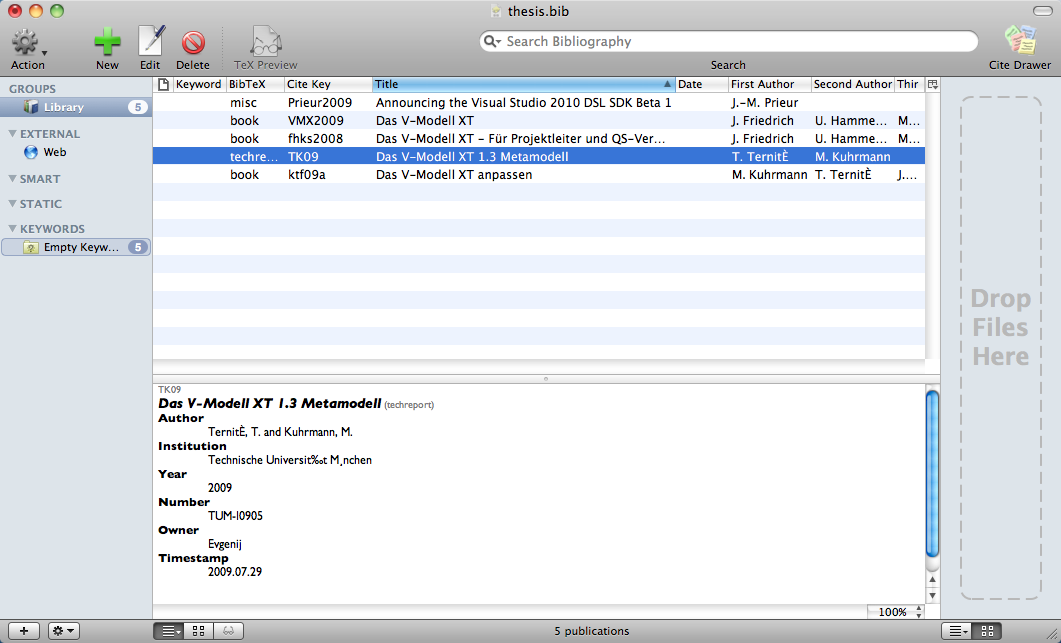
\includegraphics[width=1.00\textwidth]{imgs/bibtex.png}
	\caption{BibTeX-File f\"ur diese Vorlage}
	\label{fig:bibtex}
\end{figure}

Nebenbei zeigt der letzte Abschnitt gleichzeitig, wie eine Abbildung in die Arbeit eingebunden wird. Eine Skalierung dieses Bildes, \zB\ auf die halbe Breite des Textes und zentriert sieht dann so aus, wie in Abbildung~\ref{fig:bibtex2} dargestellt.

\begin{figure}[htbp]
	\centering
	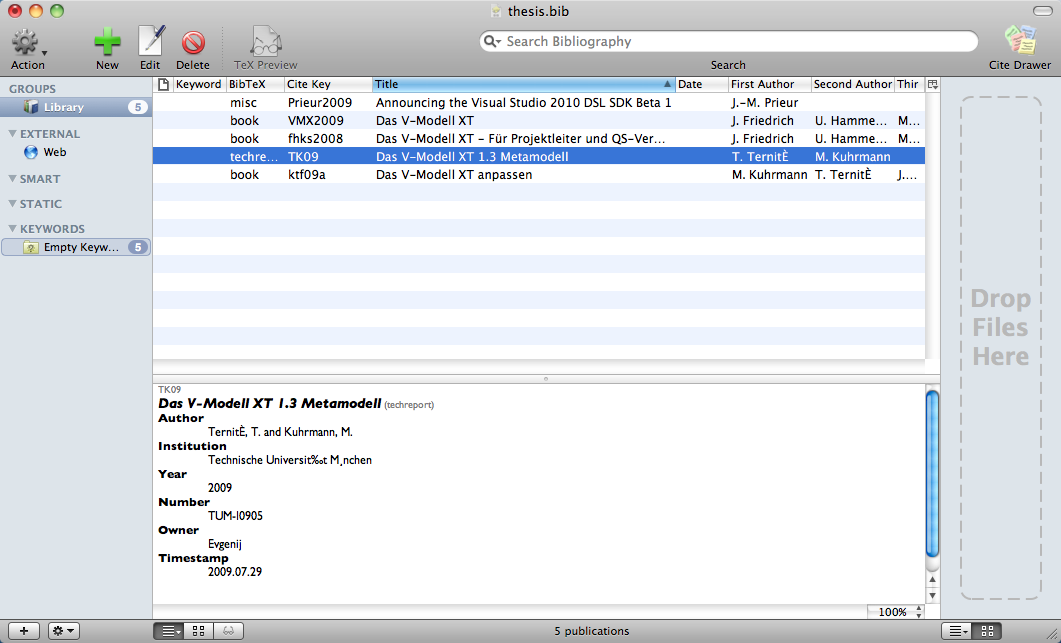
\includegraphics[width=0.5\textwidth]{imgs/bibtex.png}
	\caption[Alternativtext]{BibTeX-File f\"ur diese Vorlage -- nun in Klein}
	\label{fig:bibtex2}
\end{figure}

\begin{MySugg}
	Zu beachten ist bei Abbildungen als grobe Richtschnur: Das gr\"o{\ss}te Zeichen in der Abbildung sollte nicht gr\"o{\ss}er erscheinen, als das gro{\ss}e \emph{A} im ,,Abbildung'' der Bildunterschrift.
\end{MySugg}

Nebenbei war gerade zu sehen, wie ein spezielle Umgebung f\"ur Hinweise im Flie{\ss}text aussieht. Zur Anwendung kommt die Umgebung \kw{MySugg}, die in der Datei \kw{commands.tex} definiert ist. Ebenso gibt es dort die Umgebungen \kw{MySample} und \kw{MyBox}. Diese und die anderen Definitionen in der Datei helfen, viele Aufgaben etwas zu vereinfachen und die Ausgaben etwas aufzuh\"ubschen.

Weiterhin treten recht h\"aufig Aufz\"ahlungen und Listen auf. In dieser Vorlage ist das Paket \emph{paralist} eingebunden, das die Umgebungen \kw{compactitem} und \kw{compactenum} enth\"alt. Ein Beipiel f\"ur eine ,,klassische'' Liste ist:

\begin{itemize}
	\item Item 1
	\item Item 2
	\item Item 3
\end{itemize}

Mit der neuen Umgebung wird nicht mehr soviel Platz verschwendet, weshalb wir diese empfehlen:


\begin{compactitem}
	\item Item 1
	\item Item 2
	\item Item 3
\end{compactitem}


\section{Tabellen}
\label{sec:Tabellen}
Und so sehen die ,,h\"ubschen'' Tabellen aus\ldots

\begin{table}[htbp]
\begin{tabularx}
	{\linewidth}{@{}!{\color{white}\vrule}>{\hspace{0mm}}lL<{\hspace{0mm}} !{\color{white}\vrule width 0pt}@{}}
	\opentableheader	%\toprule
		\hl{Element} & \hl{Beschreibung} \\
	\closetableheader %\endtabularhead
		Element & Beschreibung \\
		Element & Beschreibung \\
		\midrule
		Element & Beschreibung, Beschreibung, Beschreibung, Beschreibung, Beschreibung, Beschreibung, Beschreibung, Beschreibung, Beschreibung, Beschreibung, Beschreibung\ldots \\
	\bottomrule
\end{tabularx}
  \caption[Alternativtext f\"ur das Verzeichnis]{Beispiel: Beispiel f\"ur typographisch ,,bessere'' Tabellen}%
  \label{tab:BeschreibungAllgemeinesNamensschema}
\end{table}

\begin{table}[!ht]
\begin{center}
\begin{tabular} {ll}
	\opentableheader	%\toprule
		\hl{Element} & \hl{Beschreibung} \\
	\closetableheader %\endtabularhead
		Element & Beschreibung \\
		Element & Beschreibung \\
		\midrule
		Element & Beschreibung \\
	\bottomrule
\end{tabular}
\end{center}
  \caption{Beispiel: Nicht skalierte Tabelle}%
  \label{tab:TabUnskaliert}
\end{table}

Das gro{\ss}e \emph{L} in Tabelle~\ref{tab:BeschreibungAllgemeinesNamensschema} (vgl.\ Listing~\ref{lst:TabellenCode}) sorgt daf\"ur, dass die Tabelle \"uber die gesamte Textbreite (nicht mehr und nicht weniger) skaliert. Es sogt gleichzeitig daf\"ur, dass ein automatischer Zeilenumbruch durchgef\"uhrt wird.

\begin{lstlisting}[captionpos=b, caption=Listing f\"ur die oben stehende Tabelle,label=lst:TabellenCode]
\begin{table}[htbp]
\begin{tabularx}
  {\linewidth}{@{}!{\color{white}\vrule}>{\hspace{0mm}}lL<{\hspace{0mm}} !{\color{white}\vrule width 0pt}@{}}
  \opentableheader	%\toprule
	\hl{Element} & \hl{Beschreibung} \\
  \closetableheader %\endtabularhead
	Element & Beschreibung \\
	Element & Beschreibung \\
	\midrule
	Element & Beschreibung \\
  \bottomrule
\end{tabularx}
  \caption[Alternativtext f\"ur das Verzeichnis]{Beispiel: Beispiel f\"ur typographisch ,,bessere'' Tabellen}%
  \label{tab:BeschreibungAllgemeinesNamensschema}
\end{table}
\end{lstlisting}

Soll die Tabelle~\ref{tab:BeschreibungAllgemeinesNamensschema} nicht \"uber die Seitenbreite skalieren, muss das gro{\ss}e L gegen das \"ubliche, kleine getauscht werden und es kann die ,,normale'' Umgebung \kw{table} verwendet werden. Das Aussehen zeigt die Tabelle~\ref{tab:TabUnskaliert}.

\section{Listings}
\label{sec:2:Listings}
Das Listing~\ref{lst:TabellenCode} zeigt gleichzeitig auch, wie Codefragmente mithilfe des \emph{Listings}-Paket eingebunden werden. In der Datei \kw{commands.tex} gibt es daf\"ur auch einige Makros und Hilfen, um den Umgang mit dem Paket etwas zu vereinfachen...


%%% Local Variables:
%%% mode: latex
%%% TeX-master: "thesis"
%%% End:

%\chapter{Kapitel 2 mit einigen Dingen}
\label{chp:Sonstiges}
Dieses Kapitel zeigt noch ein paar Kleinigkeiten, die f\"ur die Gestaltung der Ausarbeitung hilfreich sein k\"onnen. Insbesondere ist beschrieben, wie diese Vorlage korrekt ausgef\"ullt wird, damit man sich bei der Erstellung der Arbeit dann wirklich auf die Inhalte konzentrieren kann.

~\\
\vfill
\minitoc
\clearpage


\section{Kapitel\"ubersicht}
\label{sec:2:KapitelUebersicht}
Zu Beginn, es macht sich immer gut, Kapitel in der Arbeit strukturiert zu beginnen. Dazu ist in dieser Vorlage folgende F\"ahigkeit hinterlegt: Jedes Kapitel kann mit einer einleitenden Kurz\"ubersicht gestaltet werden, dazu ist zu Beginn jedes Kapitels der Anfang der \TeX-Datei wie in Listing~\ref{lst:KapitelCode} gezeigt zu gestalten.

\begin{lstlisting}[captionpos=b, caption=Listing f\"ur den Beginn dieses Kapitels,label=lst:KapitelCode]
\chapter{Kapitel 2 mit einigen Dingen}
\label{chp:Sonstiges}
Dieses Kapitel zeigt noch ein paar Kleinigkeiten, die f\"ur die Gestaltung der Ausarbeitung hilfreich sein k\"onnen.

~\\
\vfill
\minitoc
\clearpage
\end{lstlisting}

Dies erzeugt einen kurzen einleitenden Text f\"ur das Kapitel mitsamt einer kleinen \emph{Minitoc}, die einen groben inhaltlichen \"Uberblick gibt.

\begin{MySugg}
	Obwohl f\"ur jedes Kapitel die weiter oben beschriebenen Einleitungen inkl.\ Kapitel\"ubersicht m\"oglich sind, sollten Sie diese erst ab dem 2.~Kapitel verwenden und \emph{nicht} im ersten, einleitenden Kapitel.
\end{MySugg}

\section{Ausf\"ullen der Vorlage}
\label{sec:2:AusfuellenDerVorlage}
Um die Vorlage korrekt auszuf\"ullen sind nur wenige Schritte erforderlich:
\begin{compactenum}
	\item Eintragen der Metadaten f\"ur das Titelblatt
	\item Eintragen der Daten f\"ur die Arbeit
	\item Schreiben des Texts
	\item Erstellen der zusammenfassenden Texte
\end{compactenum}

% \paragraph{Metadaten fur das Deckblatt.}
% Das Deckblatt folgt den Vorgaben der Technischen Universit\"at M\"unchen. Um daf\"ur zu sorgen, dass auf diesem der Titel der Arbeit erscheint, sind in der Datei \kw{thesis.tex} einige Eintragungen zu machen, siehe Listing~\ref{lst:Deckblatt}. Die Eintragungen sollten selbsterkl\"arend sein.

\begin{lstlisting}[captionpos=b, caption=Metadaten f\"ur das Deckblatt,label=lst:Deckblatt]
%% Einfache Definitionen von Konstanten für das gesamte Dokument.
%  Sie werden bspw. beim Aufbau der Titelseite ausgewertet.
\def\titelname    {Name der Arbeit}
\def\autorforinfo {Marco Kuhrmann}
\def\email        {kuhrmann@in.tum.de}
\def\subjectname  {Prozessmodellierung}	%Beispiel
\def\location     {M�nchen}
\def\keywordsname {V-Modell XT}			%Beispiel

%% spezifisch fuer eine MA, fuer BA etc. muss das angepasst werden
\def\doctype{Masterarbeit in Informatik}
\def\title{The English Title}
\def\titleGer{Der Deutsche Titel (s.o.)}
\def\author{Name Autor}
\def\date{Juli 15, 2010}
\end{lstlisting}

Das Deckblatt enth\"alt nur sehr wenige Daten. \"Ublicherweise wird dieses auf Karton gedruckt, der dann als Mantel f\"ur die Arbeit dient.

\paragraph{Metadaten f\"ur die Arbeit.}
F\"ur die Arbeit selbst sind \"uber die Informationen hinaus noch weitere Daten relevant. Insbesondere die Informationen zum Aufgabensteller und zu den Betreuern sind hier zu beachten. Die betreffenden Informationen sind in der Datei \kw{titlepage.tex} (siehe Listing~\ref{lst:Deckblatt2}) einzutragen.

\begin{lstlisting}[captionpos=b, caption=Metadaten f\"ur das Deckblatt (innen),label=lst:Deckblatt2]
\vspace{20mm}
%\hfill
  \begin{tabular}{ll}
	\large Bearbeiter:      & \large \author \\[2mm]
	\large Aufgabensteller: & \large Prof. Dr. Dr. h.c. Manfred Broy \\[2mm]
	\large Betreuer:        & \large Dr. Marco Kuhrmann \\[2mm]
	\large Abgabedatum:     & \large Juni 15, 2010
  \end{tabular}
\end{lstlisting}

Auch hier sind die Eintragungen selbsterkl\"arend. Wichtig: F\"ur den Titel m\"ussen hier keine erneuten Eingaben erfolgen. Dieser wird in Deutsch und Englisch aus der \kw{thesis.tex} \"ubernommen.

\paragraph{Schreiben des Texts.}
Diese Aufgabe wird wohl den meisten Teil der Zeit w\"ahrend der Abschlussarbeit in Anspruch nehmen. Hierzu lassen sich generell nur wenige Hinweise geben:
\begin{compactitem}
	\item Beginnen Sie rechtzeitig mit schreiben!
	\item Erstellen Sie zuerst eine halbwegs stabile Gliederung und sehen Sie mindestens f\"ur jedes Kapitel eine eigene \TeX-Datei vor. Wie solche Dateien eingebunden werden, sehen Sie in der Datei \kw{thesis.tex}, die als Zentraldokument f\"ur die Arbeit fungiert.
	\item Verwenden Sie wo es geht \emph{semantisches Markup}. Das sind selbstdefinierte ,,Befehle'', die Textersetzungen vornehmen. In den Dateien \kw{commands.tex} und \kw{shortcuts.tex} finden Sie viele Beispiele.
\end{compactitem}

\paragraph{Erstellen der zusammenfassenden Texte.}
In der Vorlage gibt es verschiedene, kleine Textabschnitte, die Sie noch f\"ullen m\"ussen, bzw.\ k\"onnen. Zun\"achst die obligatorische Zusammenfassung. Diese befindet sich in der Datei \kw{abstract.tex}. Es ist vorgesehen, dass die Zusammenfassung immer in Deutsch und Englisch erstellt wird -- es wird zwar nicht vorgeschrieben, aber Sie sollten es tun.

Falls Sie jemand bei der Arbeit unterst\"utzt haben sollte und Sie ihm daf\"ur danken m\"ochten, ist in der Datei \kw{acknowledgements.tex} entsprechender Platz daf\"ur vorgesehen.

Abschli{\ss}end ist in der Datei \kw{disclaimer.tex} noch die Erkl\"arung der Selbstst\"andigkeit zu finden, mit der Sie per Unterschrift erkl\"aren, die Arbeit auch selbst erstellt zu haben. Der Name wird dort aus den Einstellung in der Datei \kw{thesis.tex} automatisch \"ubernommen und das Datum wird ebenfalls automatisch bei jeder Neuerstellung des Dokuments gesetzt.

\section{Abschluss}
\label{sec:2:Abschluss}
Eigentlich war es das auch schon. Mit diesen grundlegenden Informationen und ein wenig Vorkenntnissen in \LaTeX\ sollten Sie zu einer herzeigbaren Ausarbeitung kommen.

Diese Vorlage entwickeln wir seit \emph{8 Jahren} immer Schritt f\"ur Schritt weiter. F\"ur Anmerkungen, Feedback usw.\ sind wir immer sehr dankbar. Gerne auch Verbesserungsvorschl\"age, \zB\ in Form angepasster Makros o.\"a.

%%% Local Variables:
%%% mode: latex
%%% TeX-master: "thesis"
%%% End:

%%% Add your chapter here

\chapter{Introduction}
\label{chp:Introduction}
A software product is only as good as its development process \citep{Hsia:1993}.
This process involves specifying and understanding requirements correctly as an integral part.
Research has shown that this is prone to faults which can cost additional time and money \citep{Mendez:2006} and may lead to severe project delay \citep{Femmer:2014}.
It is therefore desirable to avoid those drawbacks by recognizing misleading requirements at an early stage and, in the best case, by specifying them clearly before the next development step.
To resolve those one must rephrase the requirements in an unambiguous way.
However, this is non trivial since often domain knowledge is required to uncover and resolve the issues \citep{Femmer:2017}.
For example in a requirement containing \textit{vague pronouns} like "The software must include a service \textit{which} must be accessible via a user interface." it is unclear whether \textit{which} relates to \textit{The software} or \textit{service}.
Another example for a requirement defect are \textit{loopholes}.
A requirement stating that the software should be tested \textit{as far as possible} leaves the reader room for interpretation and thus is ambiguous.
The previously presented defects called \textit{vague pronouns} and \textit{loopholes} are examples for so called \textit{Requirement Smells} defined by \citet{Femmer:2017}.
If a requirement smell is fulfilled it indicates that a requirement is of insufficient quality.
Consequently, requirement smells can be used to argue about the a requirement's quality

Before one can reason about a requirement's quality, one must check whether requirement smells apply or not.
An approach to accomplish this are manual review.
According to \citet{Salger:2013}, reviews have several drawbacks.
The review must be carried out by the relevant stakeholders and they must fully understand each requirement.
Consequently, the reviewer needs domain knowledge in order to perform the reviews which makes the review more difficult to execute.
Furthermore, the result of a review depends on the reviewer him/herself \citep{Zelkowitz:1983}.
Moreover, the reviewer can be distracted by the earlier mentioned requirement smells.
Therefore, \citet{Femmer:2017} conclude that reviews are costly and time consuming.

Knowing reviews are costly regarding time and money, tooling which supports the requirements engineering would be beneficial for the quality assurance process.
Such tooling could support the reviewer by automatically indicating requirement smells and therefore speed up reviews.
Further, in reality not only dedicated requirement smells are of interest, but more general speaking ambiguous or vague requirements.
Such an assistant tool should be capable to process natural language since requirements are mostly formulated in natural language \citep{Mich:2004} and indicate whether a requirement is vague or not.

Machine Learning (ML) achieved in recent history remarkable results for natural language processing (NLP) tasks \citep{Khan:2016}.
An example to mention is Google's neural network (NN) model called BERT which showcased how NNs can improve performance in transfer learning tremendously \citep{Devlin:2018}.
This recent success shows that NNs have great potential in transfer learning and consequently in detecting vague requirements.

The aim of this thesis is to further explore the potential of modern NNs in the context of detection of vague requirements.
I want to contribute the following points.
\begin{compactenum}
	\item Item 1
	\item Item 2
	\item Item 3
\end{compactenum}


% ## Struktur
%  1. Einleitung
%     1.1 Motivation: Bugs teuer und testen auch teuer
%     1.2 Problem: Vor dem release/testbaren System wissen wo bugs sind und ist der algo geeignet
%     1.3 Mein Beitrag: Implementierung und ob Algo wirkt
%     1.4 Warum löst das das Problem? Weil Studie systematisch durchgeführt 1 Seite
%   1. Abstract
%     Jeder der Punkte auf 1 bis zwei Sätze zusammengefasst
%  1. Fundamentals/Grundlagen: Erklärungen, Definitionen 2/3 Seiten
%    1.1 Was ist bug prediction
%    1.2 was ist ein linear classifier
%    1.3 Ansatz Algo für Bug-prediction erklären
%  1. Related Work (Pro Quelle ein Absatz) 7 bis 10 Papiere
%      1. Studien über bug prediction nur statisch hard gecodede Muster (google scholar)
%  (1. Approach) wie ich classifier traniere
%  1. Studie (eigentlicher Beitrag der ARbeit)
%      1.1 Ziel der Studie (Forschungsfragen)
%          Forschungsfragen(Funktioniert der Algorithmus)
%      1.1 Studie design (Vorgehen)
%          1.1 git auschecken
%          1.2 Algo drauf loslassen
%          1.3 Selbst korrigieren
%          1.4 Präzision bestimmen ("Frage 1 wird beantwortet mit folgender Metrik(Formel)")
%  1. Studie Objekts (besser mehrere)
%      1.1 Welche Repos habe ich verwendet
%      1.3 Wieviele Commits welche programmiersprache wieviele devs wieviele lines of code
%      Tabelle mit Charakteristika
%  (1. Studie exekution)
%  1. Studie Results (gegliedert nach Forschungsfrage)
%     1.1 nur die Zahlen keine Interpretation (recht kurz pro Studie Objekt eine Tabelle oder so)
%  1. Interpretation der Ergebnisse (Zeigen wie gescheit ich bin :D)
%     Antworten auf Forschungsfragen
%  1. Threats to Validity (Angriffspunkte auf meine Studie)
%      1. Veralgemeinerbarkeit weil nur begrenzte studie objekts oder nur eine Programmiersprache
%      1. Könnte Fehler in Algorithums
%      1. Ich könnte biased sein
%      (externe Validität interne Validität)
%      Ist kleiner Threat weil...
%  1. Schluss (Zusammenfassung von Einleitung bis Schluss)

%  Studie zwischen 5 bis 8 Seiten
%  Studie design ein Bild
%  zwischen 10 und 20 Seiten
% Ein Gedanke pro Absatz nicht mehr als 8-10 Zeilen

%\appendix
%\input{app01.tex}

% Todo:
% 1. Modell checken 15 min scharf nachdenken
% Änderungshäufigkeit kein guter Indikator

% Vortrag
% Einleitung mit Motivation
% Ansatz vorstellen
% Studie vorstellen
% Studie design
% Studie result (1. 5 bis 10 dateien sind studie objekts)
% Präzi schwierig
% Aber aufgrund der "natur der Datei"



%%\section{Literaturverzeichnis}
%% bibs...
%\nocite{*}
%\bibliographystyle{geralpha}
\bibliographystyle{plainnat}
\bibliography{thesis}
%\bibliography{bibtex}
\vfill
%\pagebreak

\end{document}
